\documentclass[preprint]{sig-alternate-2013}

%\newfont{\mycrnotice}{ptmr8t at 7pt}
%\newfont{\myconfname}{ptmri8t at 7pt}
%\let\crnotice\mycrnotice%
%\let\confname\myconfname%

%\permission{Permission to make digital or hard copies of all or part of this work for personal or classroom use is granted without fee provided that copies are not made or distributed for profit or commercial advantage and that copies bear this notice and the full citation on the first page. Copyrights for components of this work owned by others than ACM must be honored. Abstracting with credit is permitted. To copy otherwise, or republish, to post on servers or to redistribute to lists, requires prior specific permission and/or a fee. Request permissions from permissions@acm.org.}
%\conferenceinfo{WebSci'14,}{June 23--26, 2014, Bloomington, IN, USA.}
%\copyrightetc{Copyright 2014 ACM \the\acmcopyr}
%\crdata{978-1-4503-2622-3/14/06\ ...\$15.00.\\
%http://dx.doi.org/10.1145/2615569.2615686}
%\clubpenalty=10000 
%\widowpenalty = 10000



\usepackage{multirow}
\usepackage{dblfloatfix}
\usepackage{booktabs}
\usepackage{url}
\usepackage[font={small}]{caption, subfig}

\newcommand{\superscript}[1]{\ensuremath{^{\textrm{#1}}}}
%
\def\sharedaffiliation{%
\end{tabular}
\begin{tabular}{c}}
%


\begin{document}
	\def\cogs{\superscript{1}}
	\def\cmu{\superscript{2}}
%
% --- Author Metadata here ---
%\conferenceinfo{WebSci}{'14 Bloomington, IN USA}
%\CopyrightYear{2007} % Allows default copyright year (20XX) to be over-ridden - IF NEED BE.
%\crdata{0-12345-67-8/90/01}  % Allows default copyright data (0-89791-88-6/97/05) to be over-ridden - IF NEED BE.
% --- End of Author Metadata ---

\title{Do tags really functions as retrieval aids?}%\titlenote{For the full version of this paper, see\\ \url{https://dl.dropboxusercontent.com/u/625604/papers/Lorince.Joseph.Todd.SBP2015.pdf}}}

%
% You need the command \numberofauthors to handle the 'placement
% and alignment' of the authors beneath the title.
%
% For aesthetic reasons, we recommend 'three authors at a time'
% i.e. three 'name/affiliation blocks' be placed beneath the title.
%
% NOTE: You are NOT restricted in how many 'rows' of
% "name/affiliations" may appear. We just ask that you restrict
% the number of 'columns' to three.
%
% Because of the available 'opening page real-estate'
% we ask you to refrain from putting more than six authors
% (two rows with three columns) beneath the article title.
% More than six makes the first-page appear very cluttered indeed.
%
% Use the \alignauthor commands to handle the names
% and affiliations for an 'aesthetic maximum' of six authors.
% Add names, affiliations, addresses for
% the seventh etc. author(s) as the argument for the
% \additionalauthors command.
% These 'additional authors' will be output/set for you
% without further effort on your part as the last section in
% the body of your article BEFORE References or any Appendices.

\numberofauthors{4} %  in this sample file, there are a *total*
% of EIGHT authors. SIX appear on the 'first-page' (for formatting
% reasons) and the remaining two appear in the \additionalauthors section.
%
\author{
% You can go ahead and credit any number of authors here,
% e.g. one 'row of three' or two rows (consisting of one row of three
% and a second row of one, two or three).
%
% The command \alignauthor (no curly braces needed) should
% precede each author name, affiliation/snail-mail address and
% e-mail address. Additionally, tag each line of
% affiliation/address with \affaddr, and tag the
% e-mail address with \email.
%
% 1st. author
\centering
\alignauthor
Jared Lorince\cogs 
       \email{jlorince@indiana.edu}
% 2nd. author
\alignauthor
Kenneth Joseph\cmu
       \email{kjoseph@cs.cmu.edu}
\and
% 3rd. author
\alignauthor Peter M. Todd\cogs
\email{pmtodd@indiana.edu}
%
\sharedaffiliation
		\cogs\affaddr{Cognitive Science Program  }\\
		\affaddr{Indiana University, Bloomington, Indiana, USA}\\
		\cmu\affaddr{Computation, Organization, and Society Program}\\
		\affaddr{Carnegie Mellon University, Pittsburgh, PA, USA}
}

\toappear{For the full version of this paper, see\\ \url{https://dl.dropboxusercontent.com/u/625604/papers/Lorince.Joseph.Todd.SBP2015.pdf}}
\maketitle

\begin{abstract}
In collaborative tagging systems, it is generally assumed that users assign tags to facilitate retrieval of content at a later time. There is, however, little behavioral evidence that tags actually serve this purpose. Here we use a large-scale dataset from Last.fm to explore how patterns of music tagging and subsequent listening interact in an effort to determine if there exist measurable signals of tags functioning as retrieval aids. Results suggest that there exists only a small effect of tags increasing listening levels, with interesting differences in which kinds of tags are most associated with future listening. On the whole, our findings suggest that tagging generally is \emph{not} associated with future retrieval.
\end{abstract}

% A category with the (minimum) three required fields
%\category{H.1.2}{User/Machine Systems}{Human information processing}
%\category{H.3.5}{Information Storage and Retrieval}{Online Information Services---Web-based services}
%\category{H.5.3}{Information Interfaces and Presentation}{Group and Organization Interfaces---Collaborative computing, Web-based interaction}
%\category{J.4}{Social and Behavioral Sciences}{Psychology}


%\keywords{Collaborative tagging, Folksonomy, Music listening, Memory cues, Retrieval aids, Personal information management}

%\terms{Human Factors, Measurement, Theory}

\section{Introduction}
\label{sec:intro}
In social tagging systems, users assign freeform textual labels to digital content (music, photos, web bookmarks, etc.). It is widely assumed\footnote{Other researchers have propsed alternative motivations, however. Examples include personal information management, resource sharing, opinion expression, performance, and activism. See \cite{Gupta2010} for a review.} in the literature that tags serve as  presonal retrieval aids, allowing users to re-find content to which they have applied a given tag (e.g. a user could click on or search for the tag ``rock'' to retrieve the songs she has previously tagged with that term). This assumption is intrinsic to Vander Wal's original defintion of a folksonomy, which he contends ``is the result of personal free tagging of information and objects...\emph{for one's own retrieval}'' \cite[emphasis added]{VanderWal2007}. This perspective is echoed in many studies of tagging patterns. Is this assumption valid?
% \cite{Glushko2008,Halpin2007,Golder2006}.

Collaborative tagging systems are often designed, at least in part, as resource management platforms that expressly facilitate the use of tags as retrieval aids.  However, the freeform and often social nature of tagging opens up many other possible reasons for which a user might tag a resource. While there is a significant amount of non-controversial evidence for such alternative tagging motivations (sharing resources with other users, social opinion expression, etc.), the problem with the retrieval aid assumption runs deeper than there simply existing possible alternatives. There is, in fact, almost no behavioral evidence that tags are ever actually used as retrieval aids. While there is much data available on user tagging habits (i.e. which terms are applied to which resources, and when), to our knowledge there is no published research providing behavioral evidence of whether or not tags, once applied to items, actually facilitate subsequent retrieval. This is an issue largely driven by a lack of data: while a web service can in principle track a users' interaction with tags (for instance, if users use tags as search terms to find tagged content), there are no available datasets containing such information, nor can it be crawled externally by researchers.

Despite these issues, this empirical question is not intractable. While detailed information on how existing tags are utilized remains beyond our reach, an alternative approach is to examine how patterns of user interaction (in our case, music listening) with tagged versus untagged content vary. Our principal research question is whether listening patterns for tagged content are consistent with the expectation that tags serve as memory cues. If this were to be the case, we would expect to see an increase in a user's listening rate to musical artists after the user has tagged them, under the assumption that a tag facilitates retrieval and increases the chances of a user listening to a tagged artist. 

Here we test this hypothesis using a large-scale dataset \cite{Lorince2014} consisting of the complete listening and tagging histories of more than 100,000 users from the social music website Last.fm. From this dataset, we extract user-artist listening time-series, each of which represents the frequency of listening over 90 months to a particular artist by a particular user, and compare time-series in which the user has tagged the artist to those that are untagged. Specifically, we ask (a) does tagging an artist increases the probability of listening to that artist in the future, as shown by comparison of tagged versus untagged time-series? And (b) are certain tags particularly associated with increases in future listening?

\section{Analyses and results}
\textbf{\textit{Comparison of tagged and untagged time-series}} To provide a ``fair'' basis for comparing tagged and untagged data, we considered only tagged time series where a tag was applied in a user's month of peak listening to an artist, temporally aligning each to that peak month. Untagged time series were aligned in the same manner. See the full paper for additional criteria used in sampling time series for analysis

We then developed a a Generalized Additive Model (GAM) model that incorporates previous listening behavior on post-peak behavior. Our dependent variable in the regression was the logarithm of the sum of all listens in the six months after a tag has been applied, to capture the possible effect of tagging over a wide temporal window. Note, however, that qualitative results hold when testing listening for each individual month as well. Our independent variables are a binary indicator of whether or not the time-series has been tagged, as well seven continuous-valued predictors, one each for the logarithm of the sum of listens in the peak month and the six previous months.   

  \begin{figure}[t]
\centering
    \subfloat[\label{fig:curve}]{%
      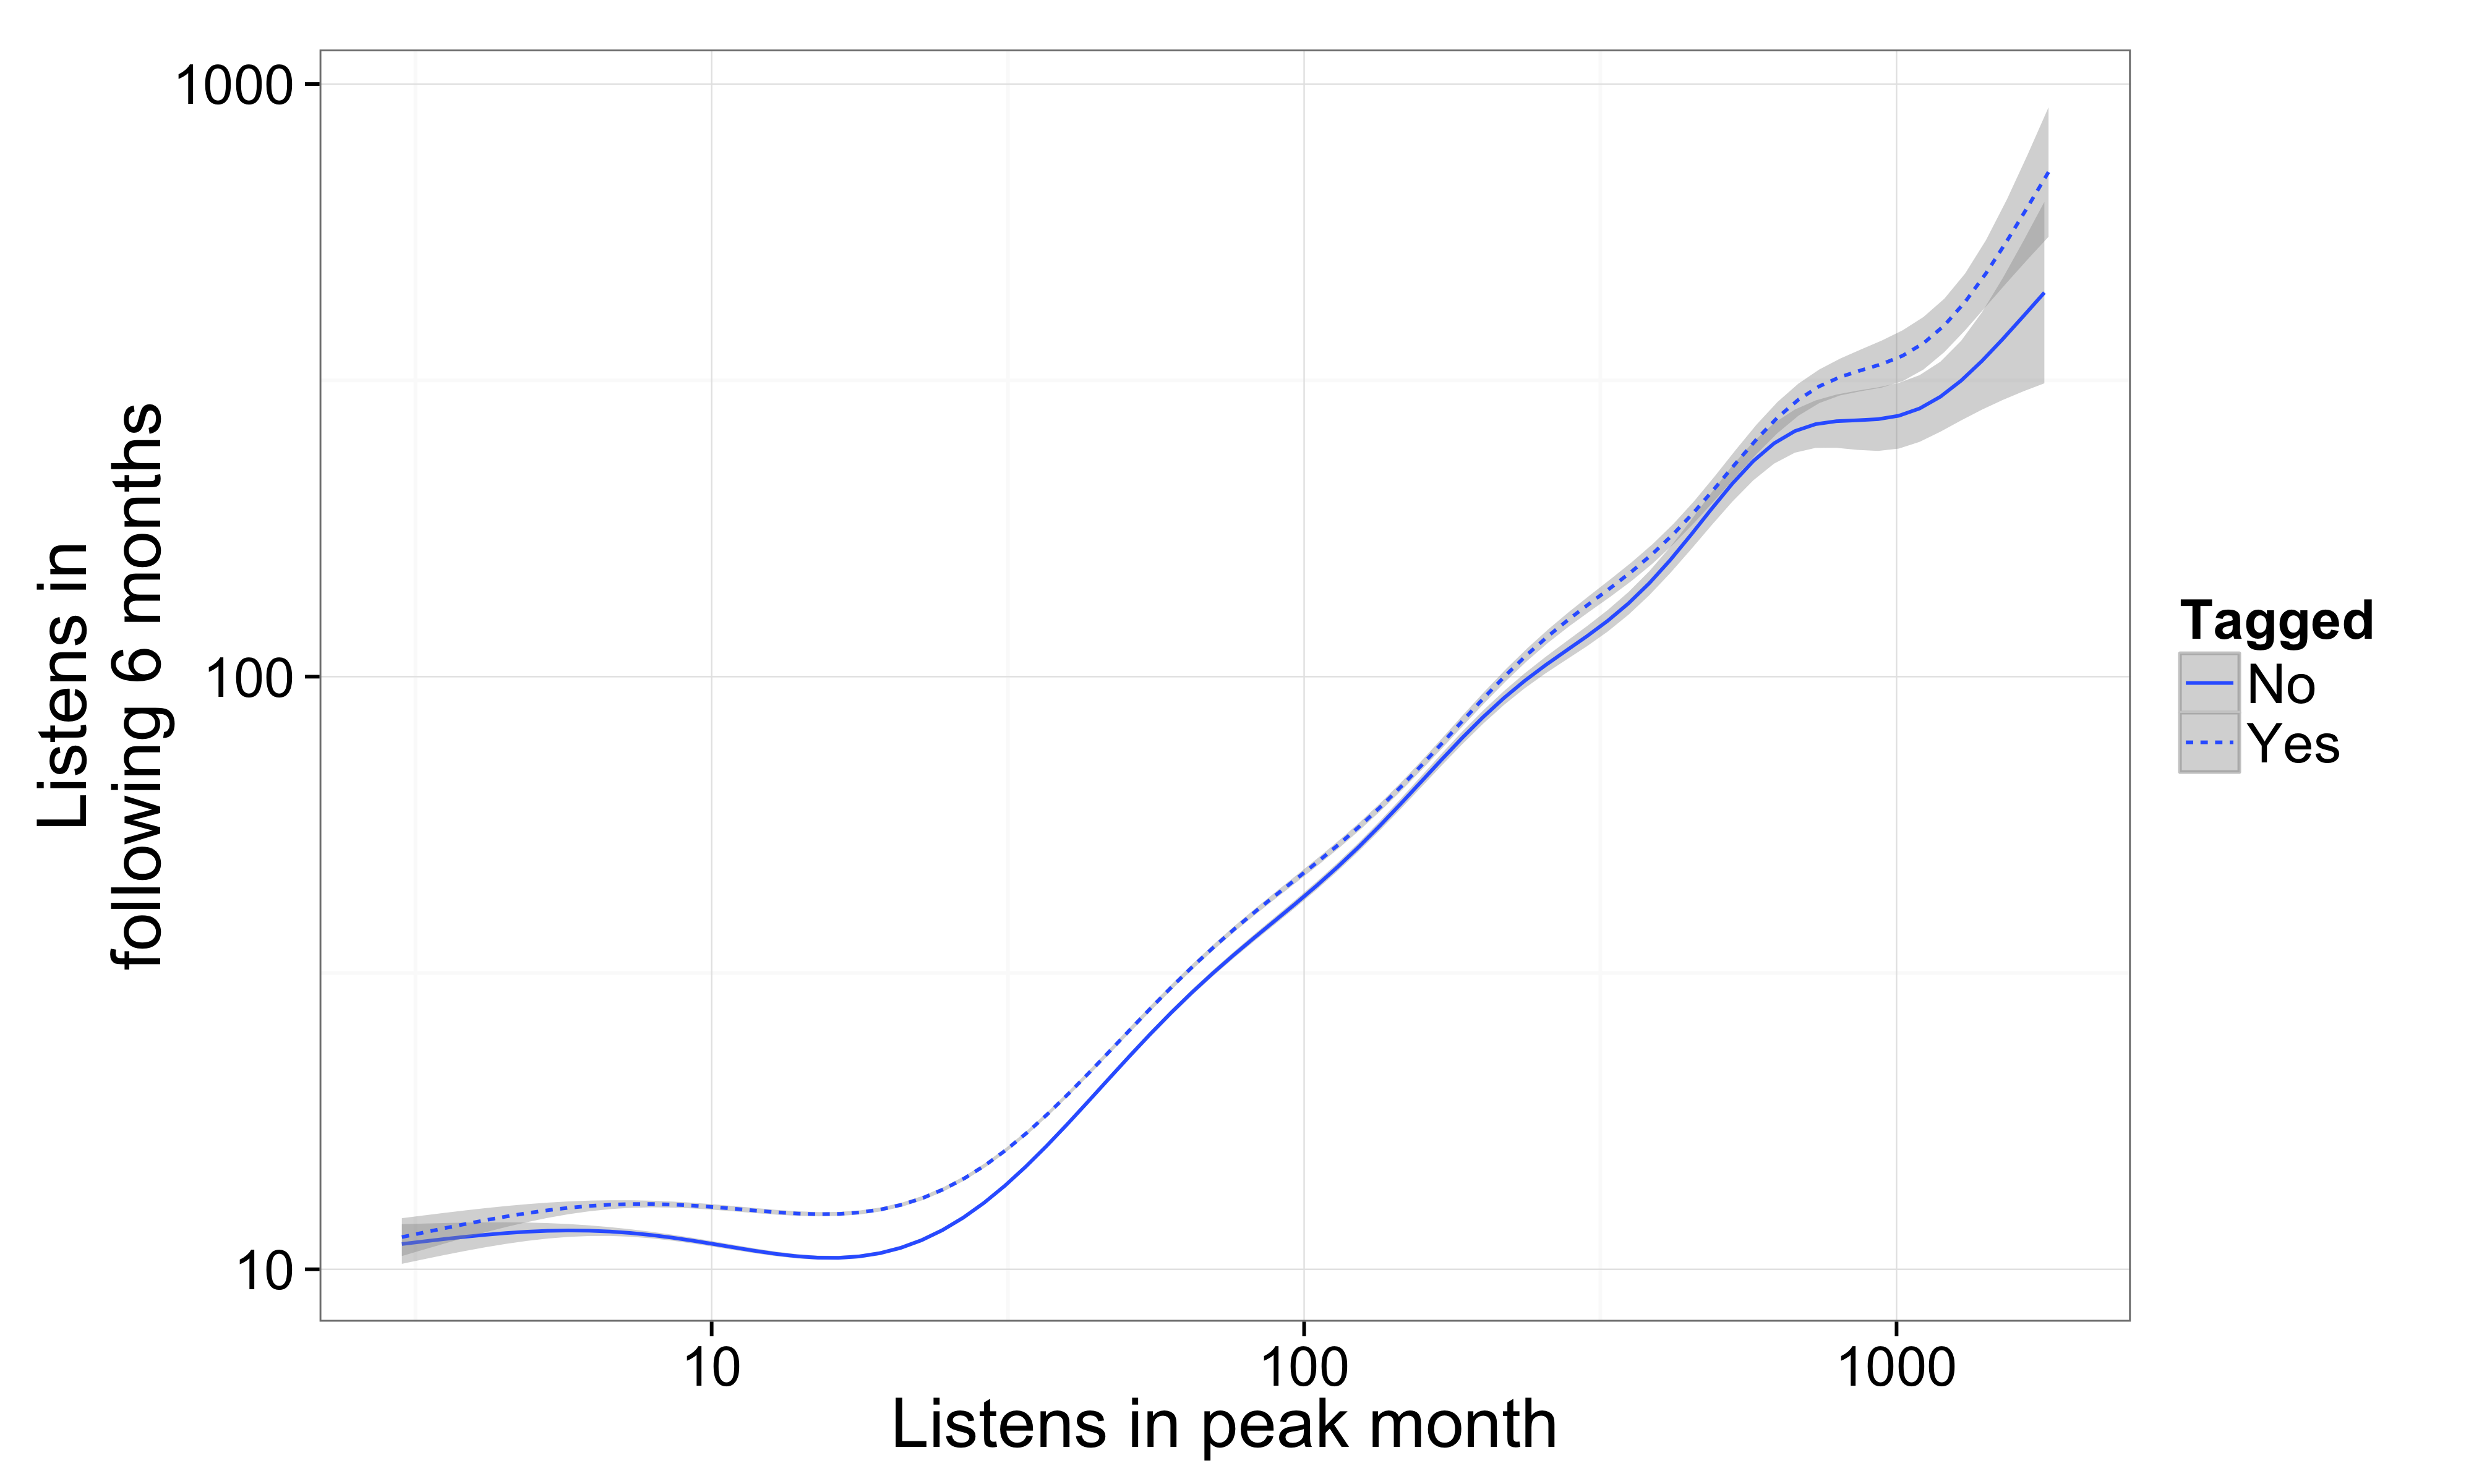
\includegraphics[width=0.4\textwidth]{taggedVUntaggedRegression.png}
    } \\

    \subfloat[\label{fig:scatter}]{%
      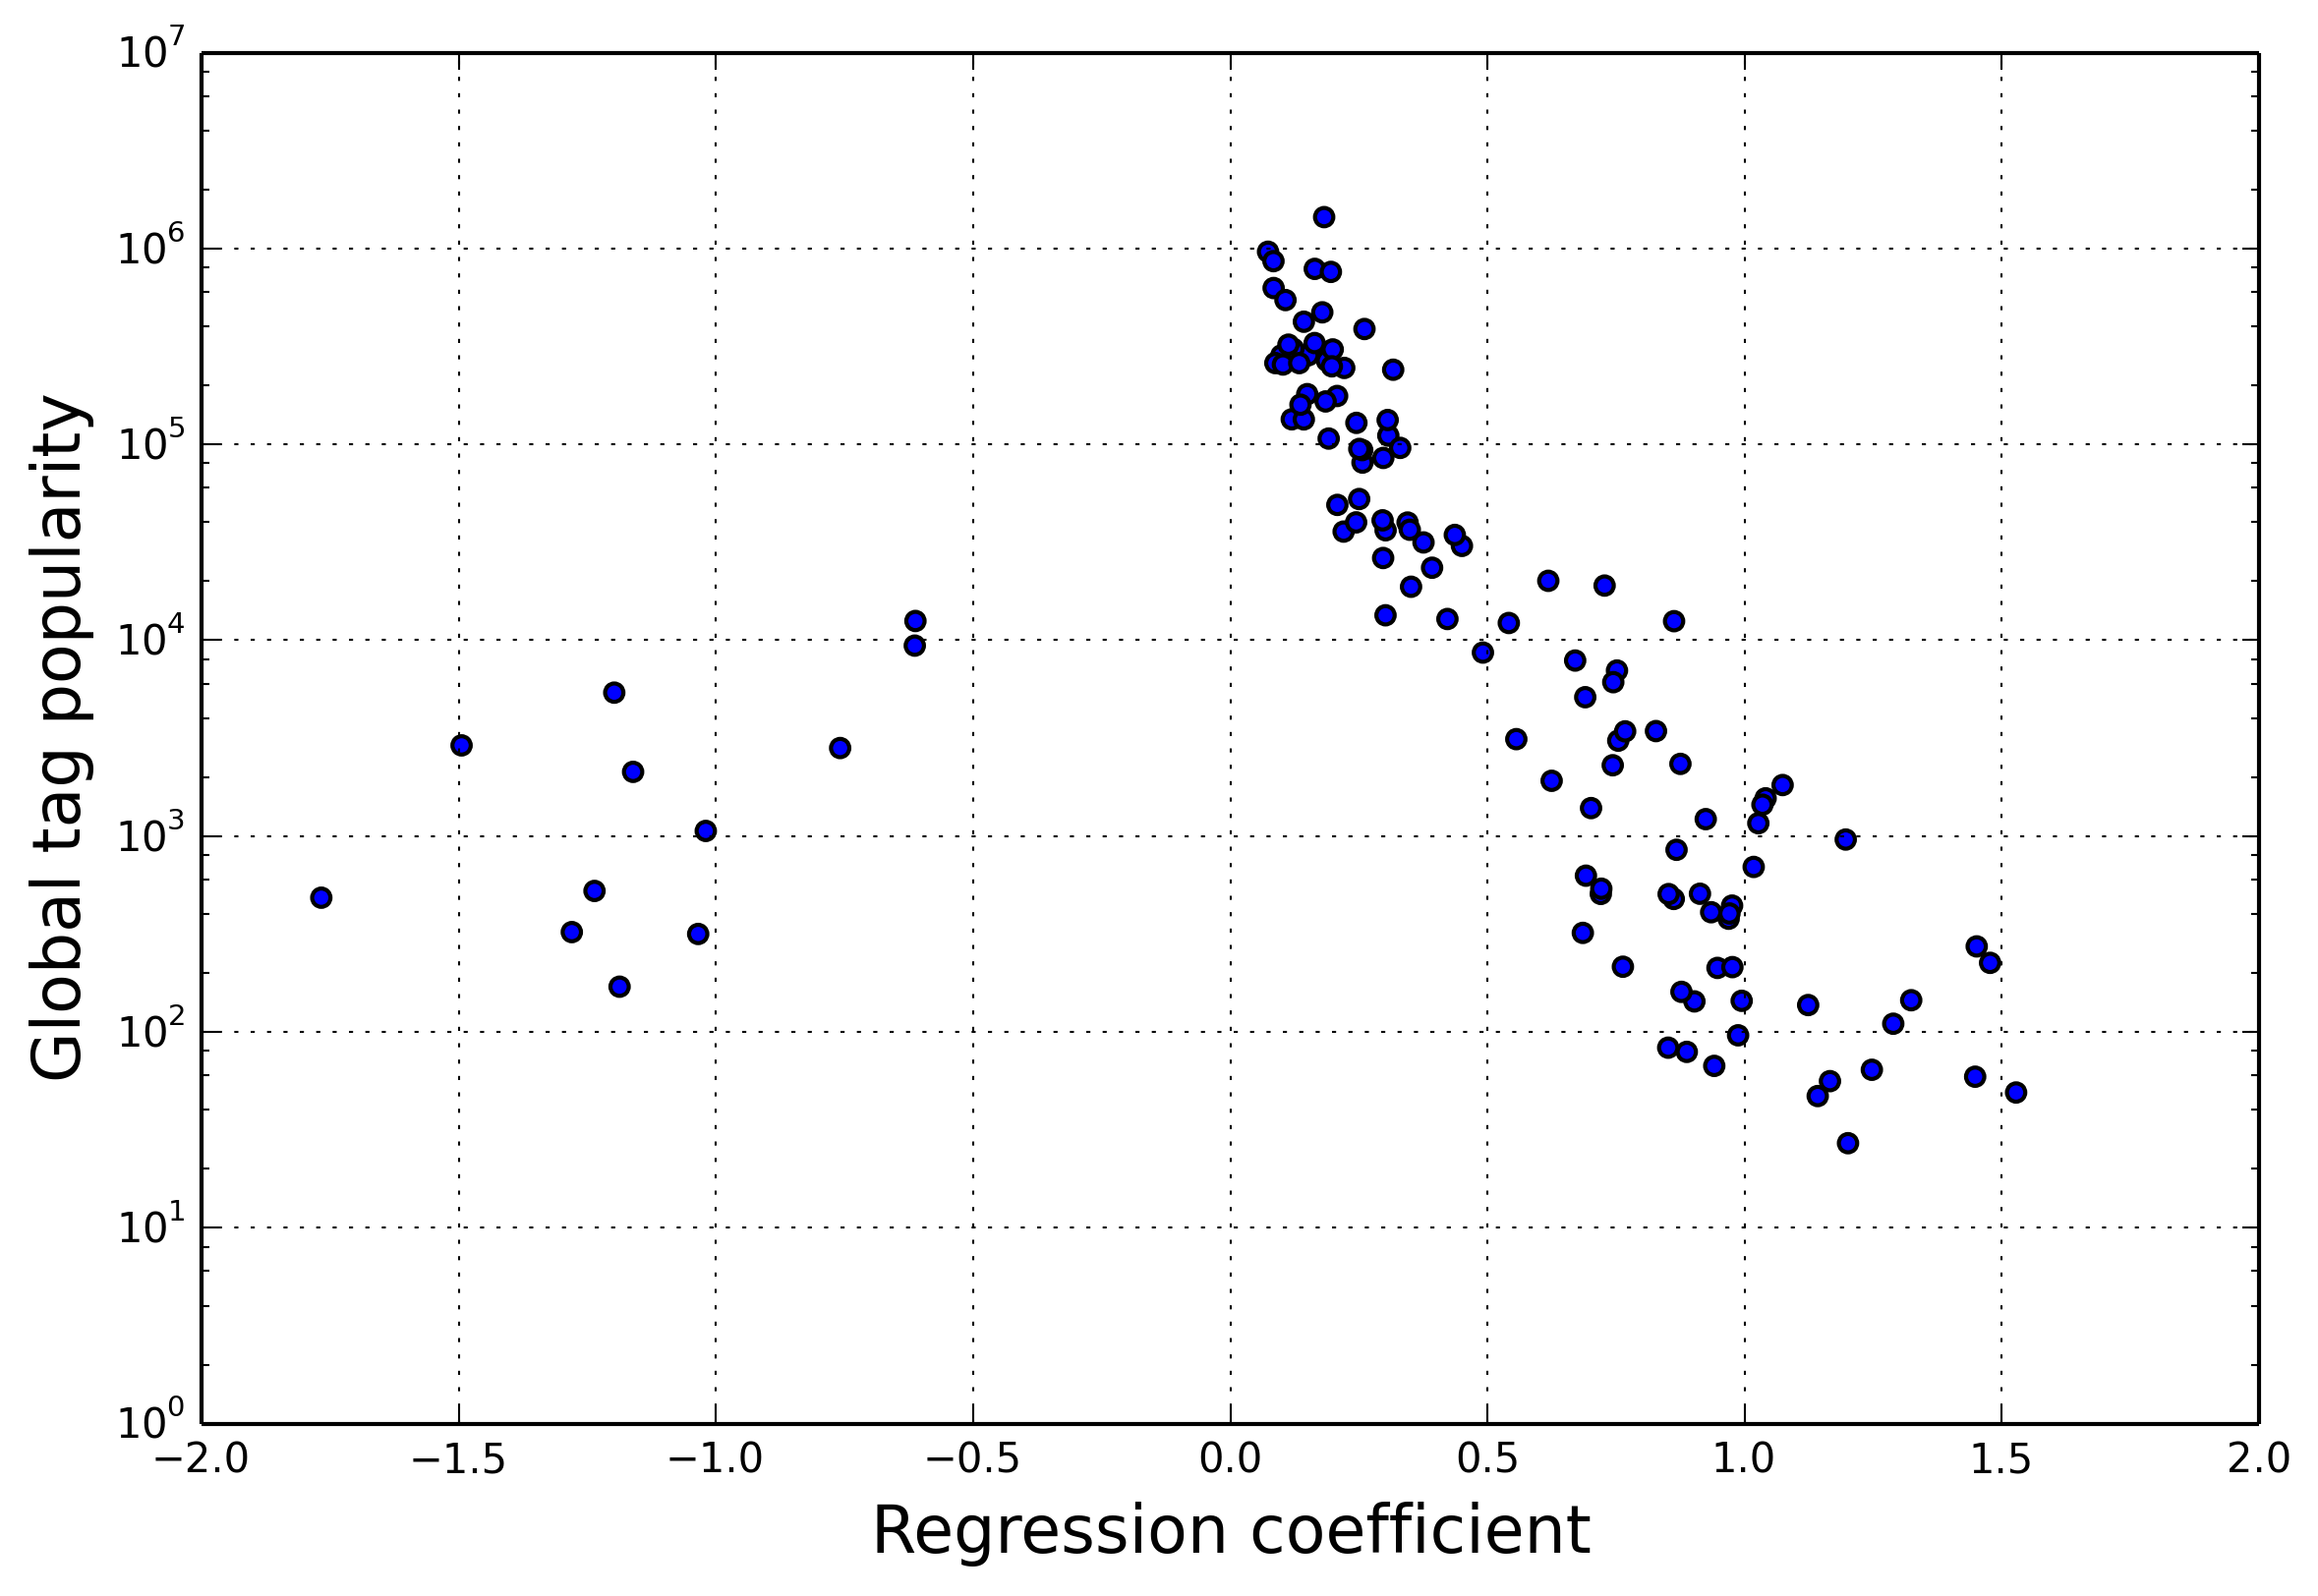
\includegraphics[width=0.35\textwidth]{c.png}
    }
   % \hfill
    %\subfloat[\label{fig:coefVsPopularityPeople}]{%
     % 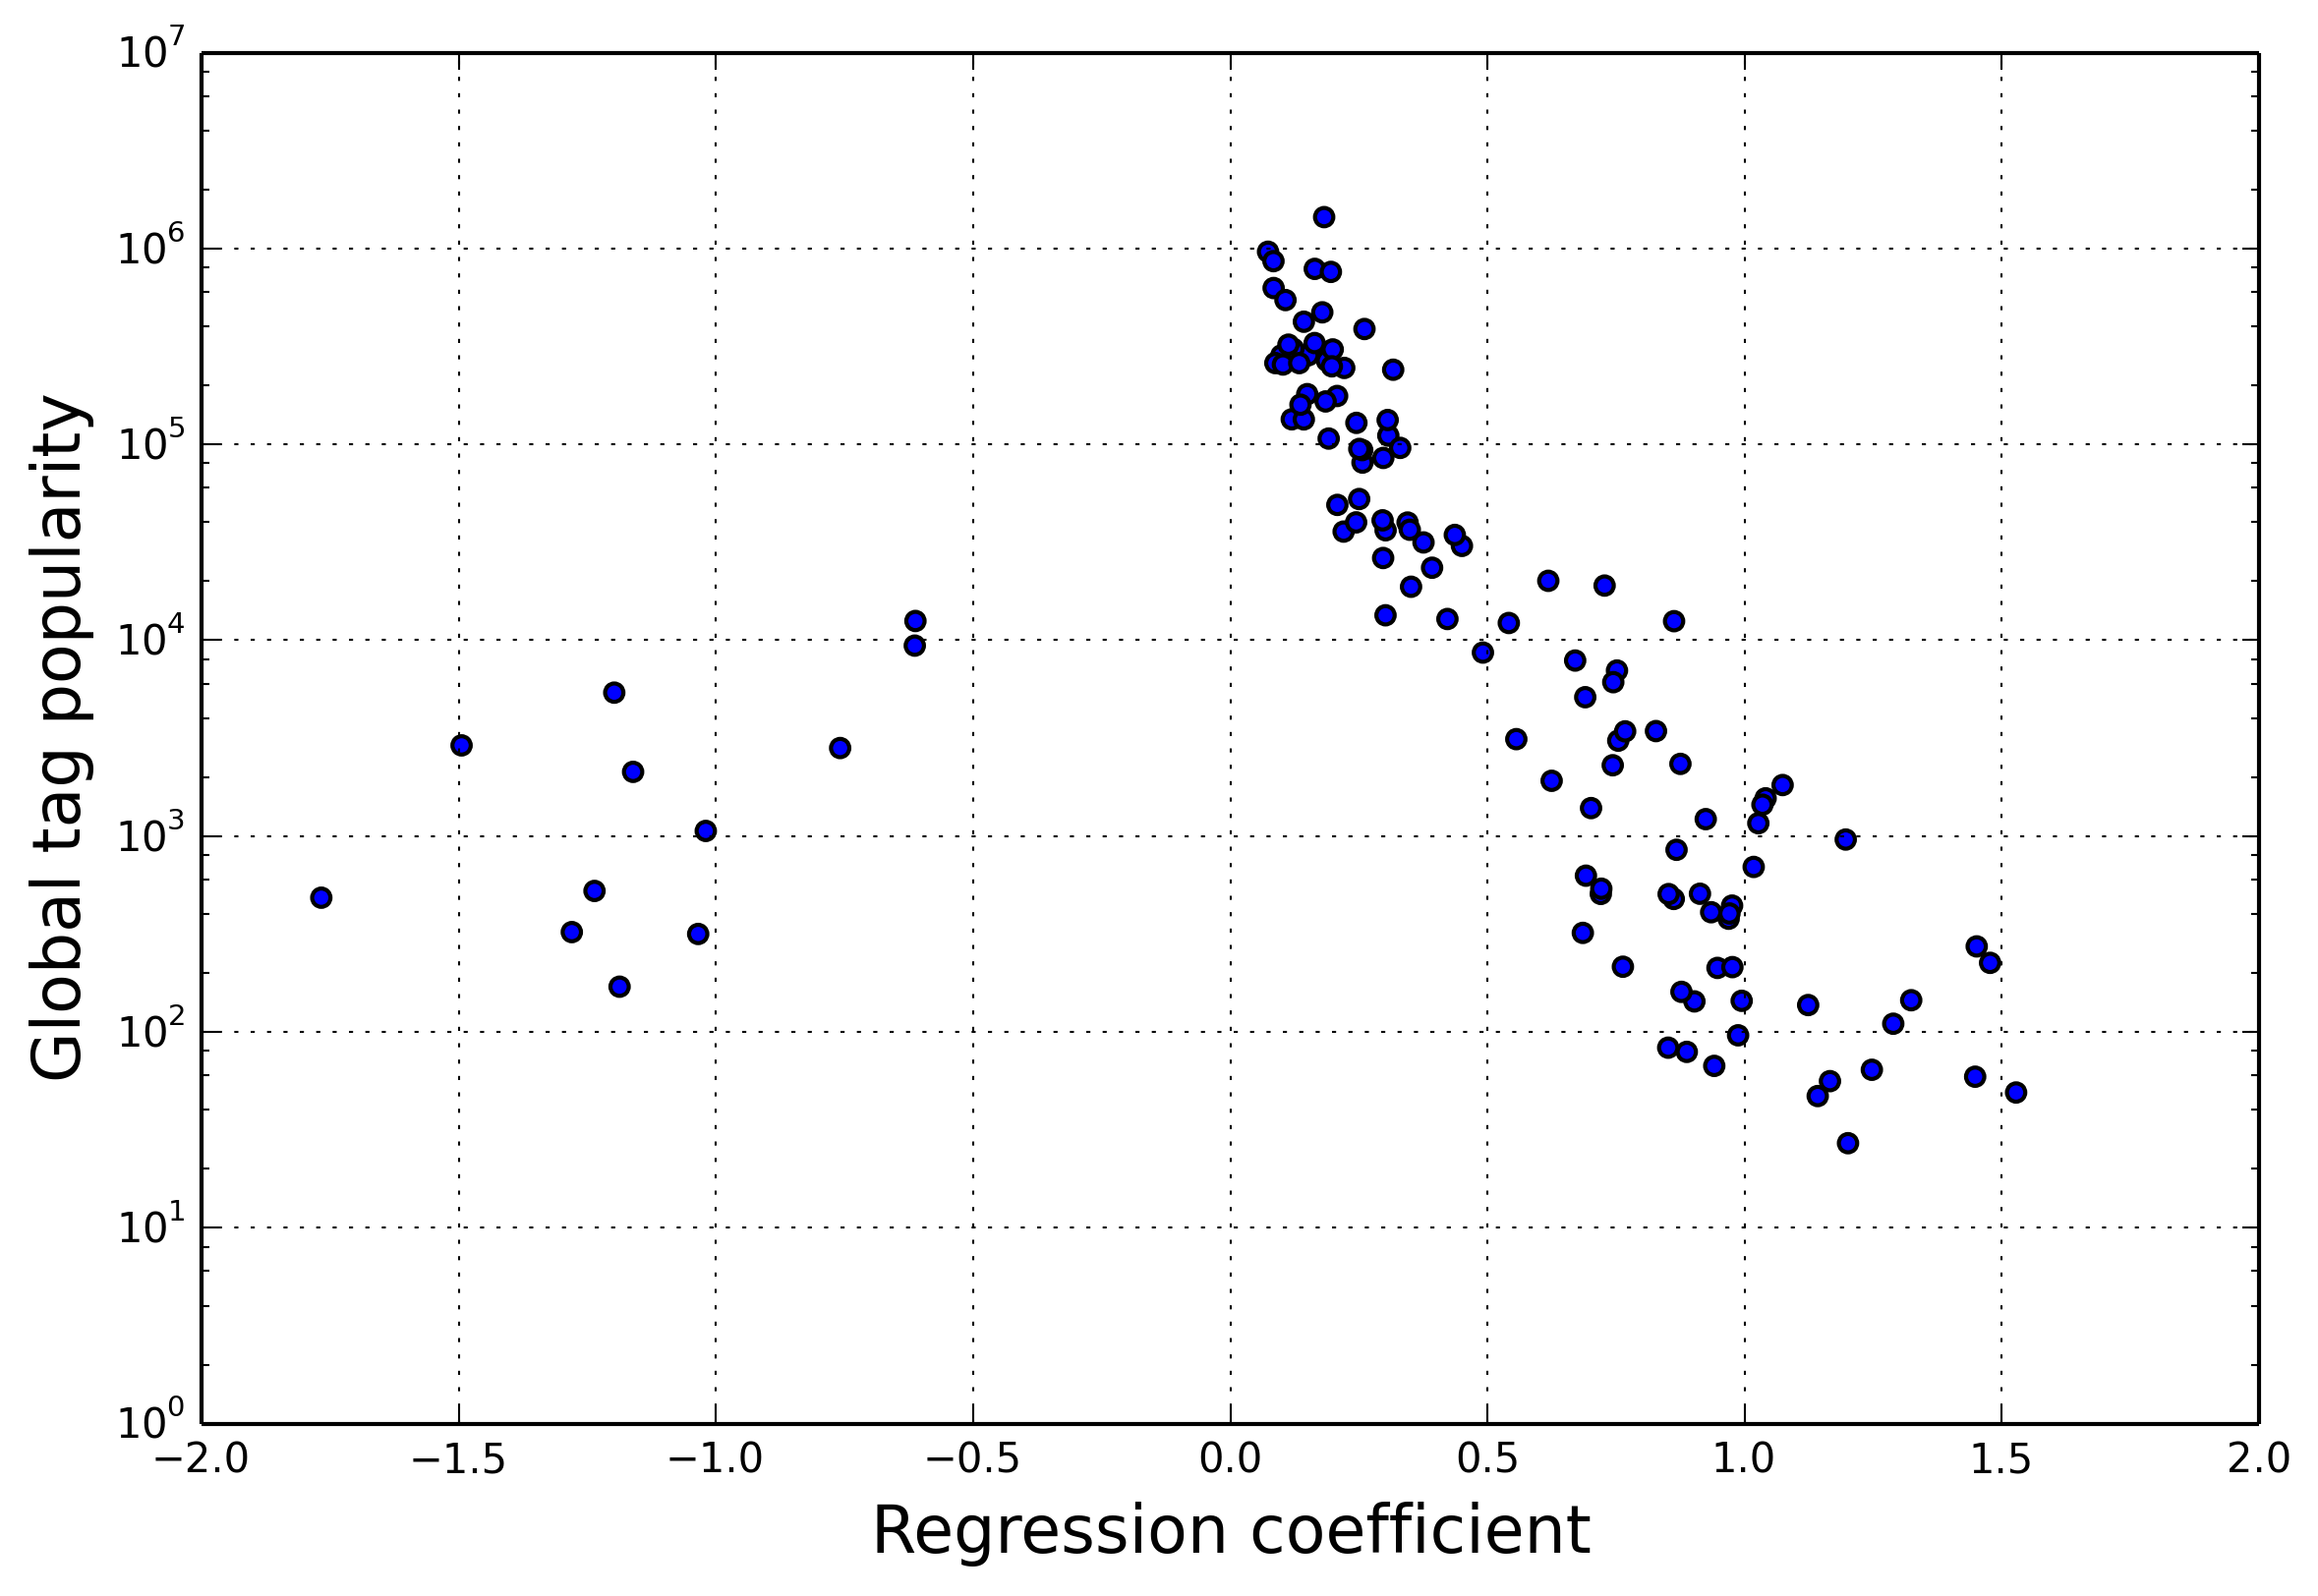
\includegraphics[width=0.3\textwidth]{c.png}
    %}
    \caption{(a): Results of regression model 1. Shown is the predicted sum of listening in the 6 months after the peak (with 95\% CI), as a function of the number of listens in the peak month. (b) Global popularity versus regression coefficient of tags in regression model 2, for the top 10\% most reliable tags in the model (in all cases $p < 0.001$).}
    \label{fig:secondPlotSet}
    \vspace{-2em}
  \end{figure}


The regression model, which explained approximately 30\% of the variance in the data (adjusted $R^{2}$), indicated that the tagged/untagged indicator, as well as listening rate parameters (smoothed using thin-plate regression splines) for all seven previous months had a significant effect on post-peak listening behavior ($P \ll 0.0001$). As we cannot show the form of this effect for all model variables at once, Figure~\ref{fig:curve} instead displays a similar model which considers only the effect of listening in the peak month on post-peak listening. As this plot suggests and the full model confirms, we can conclude that, controlling for all previous listening behavior, a tag increases the logarithm of post-peak listens by .147 (95\% CI = [.144,.150]). This indicates that the effect of a tag is associated with around 1.15 more listens over six months, on average, than if it were not to have been applied.   

\textbf{\textit{Tag analysis}} To examine if and how different tags are associated with increased future listening, we ran a regression analysis similar to that described above. Instead of a single tagged/untagged indicator, however, we included binary (present / not present) regressors for all unique tags that had at least five occurrences in our subsample

The new  mode explained approximately 29\% of the variance in the data (adjusted $R^{2}$). To address our research question, we examined which particular tags were the strongest predictors in the model. The most telling observation was that commonly-used genre tags (e.g. ``pop'', ``jazz'', and ``hip-hop'') -- which are the most common tags overall in our full dataset -- tend to be positive, but very weak predictors of future listening. In contrast, relatively strong predictors appear to be comparatively obscure, possibly idiosyncratic tags (e.g. ``cd collection'', ``mymusic'', ``purchased 09''). To examine this trend quantitatively, we plot in Figure~\ref{fig:scatter} global tag popularity as a function of a tag's impact on listening as indicated by its coefficient in the regression model. 

The data suggest that the most popular tags under both metrics considered are weak predictors of future listening, while relatively unpopular tags tend to have either strong positive or strong negative impacts on listening. 

\section{Conclusion}
This paper presents a novel methodology for testing for evidence that tagging an artist increases a user's future listening to that artist in comparison to a carefully selected set of untagged time-series. Results suggest that tagging an artist does lead to an increase in listening, but that this increase is, on average, quite small (amounting to only 1 or 2 listens over a 6 month period). Given the various possible motivations for tagging, however, we expect only some tags to serve as retrieval cues, and thus tested the relative predictiveness of future listening for different tags. This analysis revealed systematic differences in how predictive the presence or absence of different tags was for future listening as a function of tag popularity. The data suggest that, at least for the tags about which we can make statistically meaningful claims, those that are globally popular and well-known have relatively little effect on future listening. The tags that seem to ``matter'' (i.e. those that are relatively strong predictors of whether or not a user will listen to an artist after tagging it) are generally much less popular.

This suggests that, while on average tagging an artist  has a small positive effect on future listening, the most common tagging activities are \emph{not} strong predictors of future retrieval. We cannot be sure which of the many other possible tagging motivations are at play here, nor can we tell at this point if and when a tag is applied with the intention of being used for retrieval, while ultimately not being used for this purpose. That said, our results may indicate that the primary motivation for tagging on Last.fm is not for personal information management (tagging a resource for one's own retrieval), but rather may be socially oriented, resulting in tags that are useful for the community at large. This leads to the interesting possibility that a folksonomy can generate the useful, crowdsourced classification of content that proponents of collaborative tagging extol, even if this process is not strongly driven by the self-directed, retrieval-oriented tagging that is typically assumed in such systems.

%In closing, to address the titular question of whether or not tags function as retrieval aids, the best answer would appear to be ``sometimes''. While there is much work to be done on when and why particular tags serve this function and others do not, it is clear that the overarching retrieval assumption is far from universally valid: Tags certainly do not always function as memory cues, and our results suggest that retrieval may actually be an uncommon tagging motivation.

%\balancecolumns % GM June 2007
%\vfill\eject 
\bibliographystyle{abbrv}
\bibliography{references}

%\balancecolumns % GM June 2007
% That's all folks!
\end{document}
